\begin{itemize}
	\item Based on Index profile: step-index, graded index
	\item Based on made : single mode, multi mode.
\end{itemize}

\ussubsection{Step Index Single Mode}

\resizebox{\textwidth}{!}{
	\begin{tikzpicture}[thick, every node/.style={sloped,allow upside down}, font=\scriptsize]
		\begin{scope}[yshift=1.2cm, rotate=-90]
			\doubleCylinder{.5}{.15}{3}
		\end{scope}
		\draw [|-|] (-.3, -2) -- node[below] {10$\mu$m} ++(.6, 0);

		\draw [|-|] (-1, -2.8) -- node[below] {125$\mu$m} ++(2, 0);

		\begin{scope}[xshift=4cm]
			\draw (-1, -1.7) rectangle (1, 1.5);
			\draw (-.24, -1.7) rectangle (.24, 1.5);

			\draw (-1, -1) -- (-.24, -1);
			\draw (.24, -1) -- (1, -1);
			\draw (-.24, -.6) -- (.24, -.6);

			\node at (0, -.35) {$n_2$};
			\node at (-.6, -.8) {$n_1$};
			\node at (.6, -.8) {$n_1$};

			\node at (0, -2.2) {$n_1=1.45$};
			\node at (0, -2.65) {$n_2=1.46$};

			\begin{scope}[xshift=3.5cm]
				\draw[color=blue] (-1,-1) -- node {\midarrow{1pt}{.5}} (0, 0) -- ++(.7, .4) -- node {\midarrow{1pt}{.1}} ++(2, -.8) -- node {\midarrow{1pt}{.1}} ++(2, .8) -- ++(1, -.4);
				\doubleCylinder{.7}{.2}{6}
			\end{scope}
		\end{scope}
	\end{tikzpicture}
}

\begin{itemize}
	\item Allows only one path for light
	\item Bandwidth distance product: $>3 \uunit{GHzkm}$
	\item Splicing is difficut.
\end{itemize}

\ussubsection{Step Index Multi Mode}

\resizebox{\textwidth}{!}{
	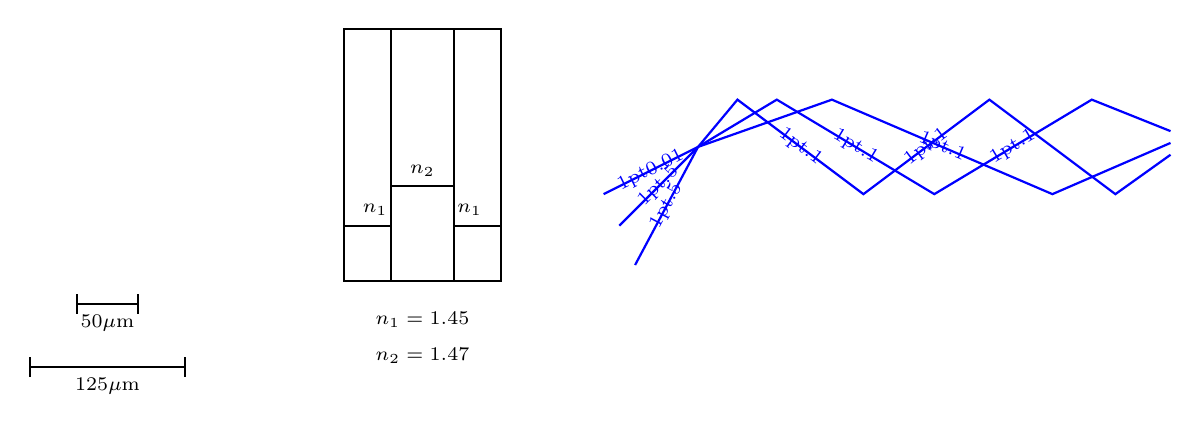
\begin{tikzpicture}[thick, every node/.style={sloped,allow upside down}, font=\scriptsize]
		\begin{scope}[yshift=1.2cm, rotate=-90]
			\doubleCylinder{.5}{.2}{3}
		\end{scope}
		\draw [|-|] (-.4, -2) -- node[below] {50$\mu$m} ++(.8, 0);

		\draw [|-|] (-1, -2.8) -- node[below] {125$\mu$m} ++(2, 0);

		\begin{scope}[xshift=4cm]
			\draw (-1, -1.7) rectangle (1, 1.5);
			\draw (-.4, -1.7) rectangle (.4, 1.5);

			\draw (-1, -1) -- (-.4, -1);
			\draw (.4, -1) -- (1, -1);
			\draw (-.4, -.5) -- (.4, -.5);

			\node at (0, -.3) {$n_2$};
			\node at (-.6, -.8) {$n_1$};
			\node at (.6, -.8) {$n_1$};

			\node at (0, -2.2) {$n_1=1.45$};
			\node at (0, -2.65) {$n_2=1.47$};

			\begin{scope}[xshift=3.5cm]
				\draw[color=blue] (-1.2,-.6) -- node {\midarrow{1pt}{0.01}} (0, 0) -- ++(1.7, .6) -- node {\midarrow{1pt}{.1}} ++(2.8, -1.2) -- ++(1.5, .65);
				\draw[color=blue] (-1,-1) -- node {\midarrow{1pt}{.5}} (0, 0) -- ++(1, .6) -- node {\midarrow{1pt}{.1}} ++(2, -1.2) -- node {\midarrow{1pt}{.1}} ++(2, 1.2) -- ++(1, -.4);
				\draw[color=blue] (-.8,-1.5) -- node {\midarrow{1pt}{.5}} (0, 0) -- ++(.5, .6) -- node {\midarrow{1pt}{.1}} ++(1.6, -1.2) -- node {\midarrow{1pt}{.1}} ++(1.6, 1.2) -- ++(1.6, -1.2) -- ++(.7, .5);
				\doubleCylinder{.7}{.3}{6}
			\end{scope}
		\end{scope}
	\end{tikzpicture}
}

\begin{itemize}
	\item Allows multiple path for light
	\item Easier to splice
	\item Bandwidth distance product (BwDP) $\sim 300 \uunit{MHz km}$
\end{itemize}

\ussubsection{Graded Index Multi Mode}

\resizebox{\textwidth}{!}{
	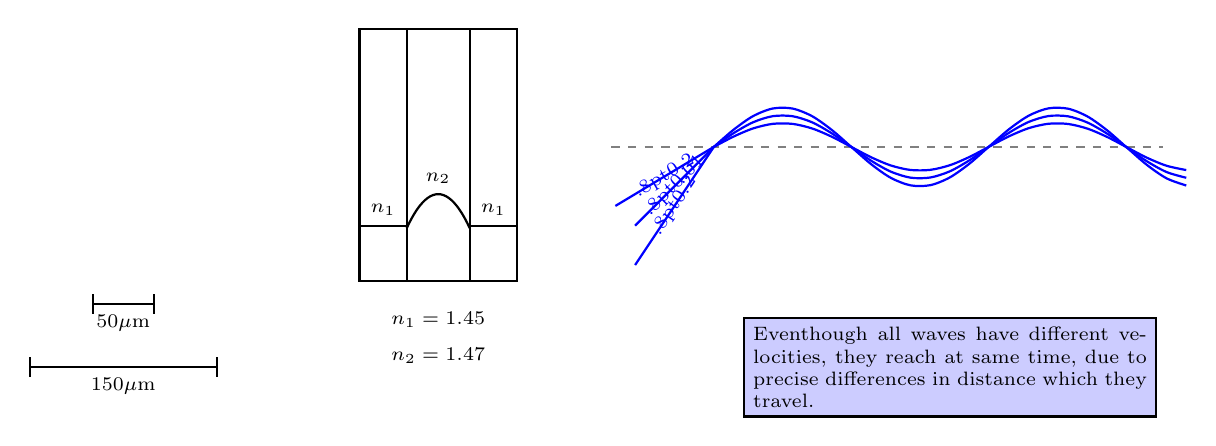
\begin{tikzpicture}[thick, every node/.style={sloped,allow upside down}, font=\scriptsize]
		\begin{scope}[yshift=1.2cm, rotate=-90]
			\doubleCylinder{.6}{.2}{3}
		\end{scope}
		\draw [|-|] (-.4, -2) -- node[below] {50$\mu$m} ++(.8, 0);

		\draw [|-|] (-1.2, -2.8) -- node[below] {150$\mu$m} ++(2.4, 0);

		\begin{scope}[xshift=4cm]
			\draw (-1, -1.7) rectangle (1, 1.5);
			\draw (-.4, -1.7) rectangle (.4, 1.5);

			\draw (-1, -1) -- (-.4, -1);
			\draw (.4, -1) -- (1, -1);
			\draw [smooth, domain=-.4:.4] plot (\x, {-\x*\x*2.7-.6});

			\node at (0, -.4) {$n_2$};
			\node at (-.7, -.8) {$n_1$};
			\node at (.7, -.8) {$n_1$};

			\node at (0, -2.2) {$n_1=1.45$};
			\node at (0, -2.65) {$n_2=1.47$};

			\begin{scope}[xshift=3.5cm]
				\draw [dashed, gray] (-1.3,0) -- ++(7, 0);
				\draw[scale=.5, domain=0:12, smooth, blue] (-2,-3) -- node {\smallmidarrow{.8pt}{0.2}} (0, 0) plot (\x, {sin(\x * .9 r)});
				\draw[scale=.5, domain=0:12, smooth, blue] (-2,-2) -- node {\smallmidarrow{.8pt}{0.01}} (0, 0) plot (\x, {.8*sin(\x * .9 r)});
				\draw[scale=.5, domain=0:12, smooth, blue] (-2.5,-1.5) -- node {\smallmidarrow{.8pt}{0.2}} (0, 0) plot (\x, {.6*sin(\x * .9 r)});
				\doubleCylinder{.7}{.3}{6}
				\node[
					draw,
					rectangle,
					fill=blue!20,
					text width=5cm,
					text justified,
					minimum height=8mm,
					xshift=3cm,
					yshift=-2.8cm
				] {Eventhough all waves have different velocities, they reach at same time, due to precise differences in distance which they travel.};
			\end{scope}
		\end{scope}
	\end{tikzpicture}
}

\begin{itemize}
	\item Gradual decrease in refractive index.
	\item BWDP $\approx 3 \uunit{GHz km}$
\end{itemize}

\ussubsection{Comparison between different Cables}

\begin{longtblr}
	{
		colspec = {XX},
		hlines,
		vlines,
		rowsep=6pt,
		colsep=5pt,
		row{1}={bg=blue!10!white}
	}

	\SetCell{c} \textbf{Step Index}                                   & \SetCell{c} \textbf{Graded Index}                               \\
	Refractive index changes sharply from core-cladding interface     & Refractive index changes gradually from core-cladding interface \\
	Refractive index profile looks like steps                         & Refractive index profile looks like parabola                    \\
	Attenuation is more for multimode and less for single mode        & Attenuation is usually less                                     \\
	Numerical Aperture is more for multimode and less for single mode & Numerical Aperture is usually less                              \\
\end{longtblr}

\begin{longtblr}
	{
		colspec = {XX},
		hlines,
		vlines,
		rowsep=6pt,
		colsep=5pt,
		row{1}={bg=blue!10!white}
	}

	\SetCell{c} \textbf{Single Mode}              & \SetCell{c} \textbf{Multi Mode}                                  \\
	Only one mode can propagate through fibre     & Allows a large number of modes                                   \\
	Smaller core diameter                         & Larger core diameter                                             \\
	Difference in refractive indices is very less & Difference in refractive indices is more compared to single mode \\
	No multimodal dispersion                      & There is multimodal dispersion
\end{longtblr}
